\newtoggle{withbonus} \toggletrue{withbonus} % set true to show bonus points in grade table

% setting underlying course name (Grundlagenfach Mathematik, §-Unterricht, \ldots)
\newcommand{\mycourse}{Grundlagenfach Informatik}
% name of the class
\newcommand{\myclass}{3. Klassen}
% set date
\newcommand{\mydate}{13. September 2024}

\title{\textbf{Hardware}}
\author{Thomas Graf\\
\mycourse, \myclass}
\date{\mydate}
\maketitle
\thispagestyle{headandfoot}		
\clearpage

\begin{questions}

\question[2]

Gib die Wertetabelle an, die durch folgende Schaltung erzeugt wird:
\begin{figure}[H]
    \centering
    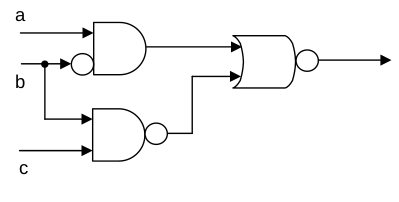
\includegraphics[scale=0.6]{EF/Exams/aufgabe01.png}
\end{figure}
Hinweis: Der \enquote{Kreis} ist eine Kurzschreibweise für einen Inverter (Negation) \begin{tikzpicture}\node[not gate US, draw] (Not1) {};\end{tikzpicture}. Bezeichne das Outputsignal in deiner Wahrheitstabelle entweder mit \textit{d} oder mit \textit{Out}.

\begin{solution}
    Die gesuchte Wahrheitstabelle (wir bezeichnen das Outputsignal mit \textit{d}) lautet:
\begin{figure}[H]
    \centering
    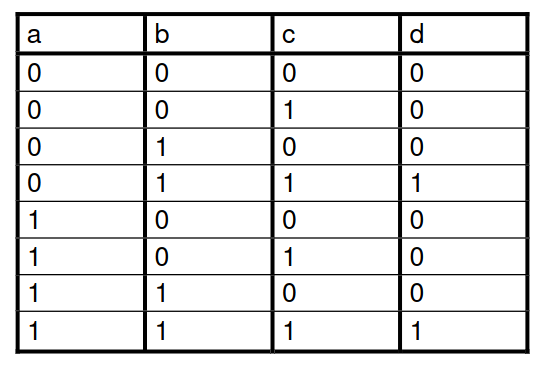
\includegraphics[scale=0.6]{EF/Exams/sol_aufgabe01.png}
\end{figure}
\end{solution}
\clearpage
\question
Betrachte die nachfolgende Abbildung.
\begin{figure}[H]
    \centering
    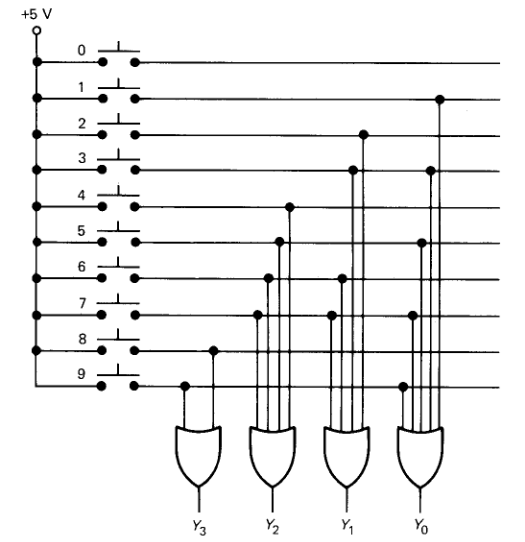
\includegraphics[scale=0.6]{EF/Exams/aufgabe02.png}
\end{figure}
Der Output dieser Schaltung ist das binäre Wort $Y_3Y_2Y_1Y_0$ der Länge 4. Bei den Ziffern 0 bis 9 ist jeweils ein Drückschalter (push-button switch) wie bei einem Taschenrechner angebracht. Wir gehen hier davon aus, dass zu jeder Zeit höchstens einer der Drückschalter gedrückt (geschlossen) wird!
\begin{parts}
    \part[1] Wie lautet das Outputwort, wenn genau der Drückschalter bei Ziffer 3 (und kein anderer) gedrückt (geschlossen) wird?
    \begin{solution}
    Das Outputwort lautet dann $0011$.
    \end{solution}
    \part[1] Wie lautet das Outputwort, wenn genau der Drückschalter bei Ziffer 5 (und kein anderer) gedrückt (geschlossen) wird?
    \begin{solution}
    Das Outputwort lautet dann $0101$.
    \end{solution}
    \part[2] Was tut diese Schaltung? Wieso / warum könnte eine solche Schaltung z.B. in einem Taschenrechner eingesetzt werden?
    \begin{solution}
    Eine solche Schaltung wird \textit{decimal-to-binary encoder} genannt. Das Drücken des Schalters gehörend zu Ziffer $n$ erzeugt ein Outputwort, welches genau der binären Darstellung der Ziffer $n$ entspricht. So wird z.B. beim Drücken vom Schalter bei Ziffer 9 das Outputwort $1001$ angenommen --- dies ist die binäre Darstellung der 9. In einem Taschenrechner kann dadurch dezimaler Userinput in das Binärsystem (zur weiteren Verarbeitung im binär arbeitenden Taschenrechner) umgewandelt werden (encoding).
    \end{solution}
\end{parts}
\droptotalpoints


\question[2]
Betrachte die Schaltung in der nachfolgenden Abbildung.
\begin{figure}[H]
    \centering
    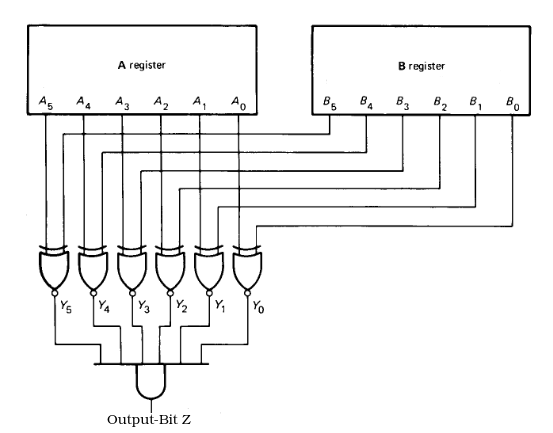
\includegraphics[scale=0.7]{EF/Exams/aufgabe03.png}
\end{figure}
Der Output dieser Schaltung ist das binäre Wort $Y_5Y_4Y_3Y_2Y_1Y_0$ der Länge 6. Die beiden Register $A$ und $B$ haben jeweils ein binäres Wort ($A_5A_4A_3A_2A_1A_0$ beziehungsweise $B_5B_4B_3B_2B_1B_0$) der Länge 6 abgespeichert. Dabei ist ein einzelnes abgespeichertes Bit mit Wert 1 als $+5$ Volt Spannung zu interpretieren und ein einzelnes abgespeichertes Bit mit Wert 0 als $+0$ Volt Spannung. Welche Bedeutung hat der Wert des Output-Bits $Z$?
\begin{solution}
Dies ist ein sogenannter \textit{word comparator}. Dieser hat den Output $Z = 1$, falls die beiden Wörter $A$ und $B$ Bit für Bit identisch sind und den Output $Z = 0$, falls sich $A$ und $B$ um mindestens ein Bit unterscheiden.
\end{solution}


\question[2]
Betrachte die Schaltung in der nachfolgenden Abbildung. In dem 8-Bit Register ist ein binäres Wort $A := A_7A_6A_5A_4A_3A_2A_1A_0$ der Länge 8 abgespeichert. Dabei ist ein einzelnes abgespeichertes Bit mit Wert 1 als $+5$ Volt Spannung zu interpretieren und ein einzelnes abgespeichertes Bit mit Wert 0 als $+0$ Volt Spannung. Der Output der Schaltung ist das binäre Wort $Y := Y_7Y_6Y_5Y_4Y_3Y_2Y_1Y_0$ der Länge 8. Die Schaltung kann gesteuert werden durch das Kontroll-Bit $K$. Welche Auswirkung hat der Wert (entweder 0 oder 1) des Kontroll-Bits $K$ auf den Output $Y$?
\begin{figure}[H]
    \centering
    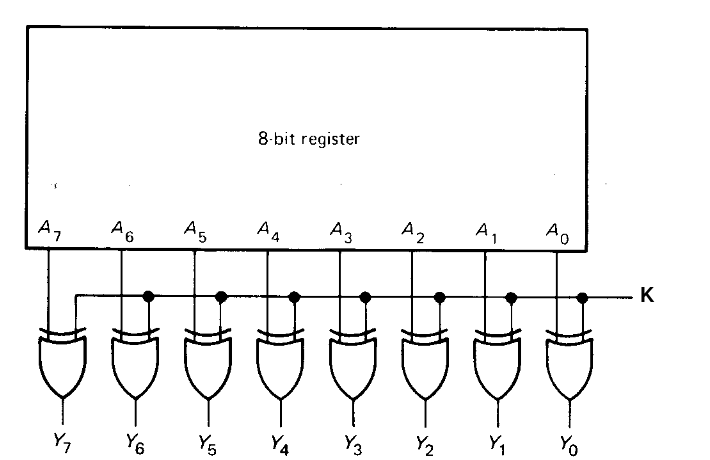
\includegraphics[scale=0.7]{EF/Exams/aufgabe04.png}
\end{figure}
\begin{solution}
Bei der Schaltung handelt es sich um einen \textit{kontrollierten Inverter}. Falls das Kontroll-Bit auf $+0$ Volt (\textit{low}) gesetzt ist, dann wird das abgespeicherte Wort direkt an den Output übertragen. In diesem Fall ($K=0$) gilt also für den Output
\begin{align*}
    Y = A.
\end{align*}
Ist das Kontroll-Bit hingegen auf $+5$ Volt (\textit{high}) gesetzt, so ist jedes Ouput-Bit $Y_n$ genau die Negation von $A_n$ (geschrieben $\bar{A_n}$), $n\in\lrc{0,1,\ldots, 7}$. Für den Output gilt dann ($K=1$) also
\begin{align*}
    Y = \bar{A} := \bar{A_7}\bar{A_6}\ldots\bar{A_0}.
\end{align*}
\end{solution}



\question[2]
\begin{figure}[H]
    \centering
    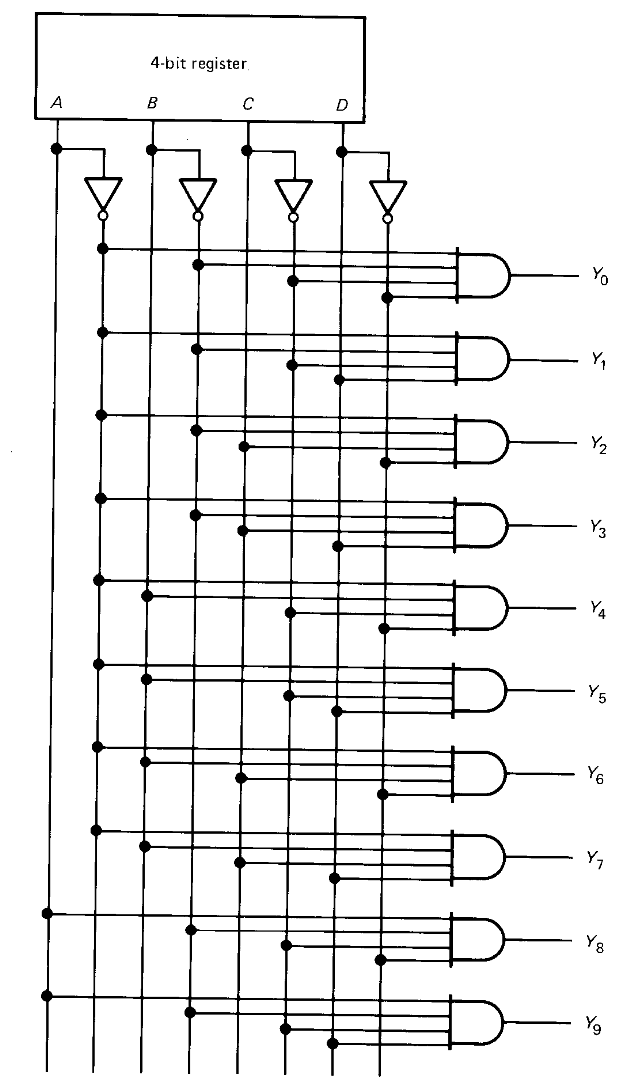
\includegraphics[scale=0.7]{EF/Exams/aufgabe05.png}
\end{figure}





\end{questions}
